\documentclass[12pt]{article}

% packages
\usepackage{kantlipsum}
\usepackage[margin=1in]{geometry}
\usepackage[labelfont=it]{caption}
\usepackage[table]{xcolor}
\usepackage{subcaption,framed,colortbl,multirow}
\usepackage{amsmath,amsthm,amssymb,wasysym,mathrsfs,mathtools}
\usepackage{tikz,graphicx,pgf,pgfplots}
\usetikzlibrary{arrows, angles, quotes, decorations.pathreplacing, math, patterns, calc}
\pgfplotsset{compat=1.16}

% custom commands
\newcommand{\N}{\mathbb{N}}
\newcommand{\Z}{\mathbb{Z}}
\newcommand{\I}{\mathbb{I}}
\newcommand{\R}{\mathbb{R}}
\newcommand{\Q}{\mathbb{Q}}
\newcommand{\C}{\mathbb{C}}
\newcommand{\F}{\mathbb{F}}
\newcommand{\p}{^{\prime}}
\newcommand{\powerset}{\raisebox{.15\baselineskip}{\Large\ensuremath{\wp}}}
\DeclarePairedDelimiter{\ceil}{\lceil}{\rceil}
\DeclarePairedDelimiter\floor{\lfloor}{\rfloor}

\setlength{\fboxsep}{4pt}
\newcommand{\exercise}[2]{\section*{Exercise #1}\begin{center}\framebox{\begin{minipage}{\textwidth-10pt}#2\end{minipage}}\end{center}}
\newcommand{\problem}[2]{\section*{Problem #1}\begin{center}\framebox{\begin{minipage}{\textwidth-10pt}#2\end{minipage}}\end{center}}
\newcommand{\generic}[2]{\section*{#1}\begin{center}\framebox{\begin{minipage}{\textwidth-10pt}#2\end{minipage}}\end{center}}

 
\begin{document}
 
\title{Assignment 3\\
    \large MATH CS 120FG Graph Theory I}
\author{Harry Coleman}
\date{February 6, 2020}
\maketitle

\exercise{1}{
    For which $n$ is the hypercube $Q_n$ planar?
}

Since each $Q_n$ is a subgraph of $Q_{n+1}$, we want to find the largest $n$ such that $Q_n$ is planar, which will tell us that $Q_k$ is planar if and only if $0\leq k \leq n$. Since hypercube graphs are bipartite, they are triangle free. So each hypercube is a simple complete triangle-free graph, and is planar if and only if
\[e \leq 2v - 4.\]
For $Q_3$, there are 8 vertices, and 12 edges, so since
\[12 \leq 2\cdot 8 - 4 = 12,\]
$Q_3$ is planar. For $Q_4$, there are 16 vertices and 32 edges, so since
\[32 > 2\cdot16 - 6 = 16,\]
$Q_n$ is nonplanar for all $n\geq4$ and planar, otherwise.


\exercise{2}{
    If $G$ has at least 11 vertices, prove that $G$ and its complement $\overline{G}$ cannot both be planar.
}

Suppose $G$ is a simple planar graph on $v\geq$ vertices. If $G$ is connected, then
\[e(G) \leq 3v - 6.\]
If $G$ is not connected, we have components $C_1,\dots,C_k$. For each pair $C_i,C_{i+1}$ with $1\leq i \leq k-1$, we add an edge from an external vertex in $C_i$ to an external vertex in $C_{i+1}$, such that the graph remains planar. Call this new connected simple planar graph $G`$. Since $G$ has fewer edges than $G`$ and $G`$ is a connected simple planar graph,
\[e(G) < e(G') \leq 3v-6.\]
So
\[e(G) \leq 3v-6\]
whether $G$ is connected or not. We now consider the complement of $G$. Since an edge $(u,v)\in V(\overline{G})$ if and only if $(u,v)\notin V(G)$, then every possible edge between vertices is either in $G$ or $\overline{G}$. Since there are
\[\binom{v}{2} = \frac{v!}{(v-2)!2!} = \frac{v(v-1)}{2}\]
possible edges, we must have
\[\frac{v(v-1)}{2} = e(G) + e(\overline{G}).\]
And by the inequalities we found,
\[\frac{v(v-1)}{2} = e(G) + e(\overline{G}) \leq 3v-6 + 3v-6,\]
\[v(v-1) \leq 12v-24,\]
\[v^2 - 13v + 24 \leq 0,\]
\[v \leq 10.772... < 11.\]
So if $G$ and $\overline{G}$ are both simple planar graphs, then $v<11$. So if $V\geq11$, then $G$ and $\overline{G}$ are not both simple planar graphs.

\exercise{4}{
    Suppose $G$ is a 3-regular simple planar graph where each face is a 5-cycle. Calculate the number of vertices, edges and faces of $G$.
}

The degree of each vertex is 3 and the length of each face is 5. So if $v$ is the number of vertices, $f$ is the number of faces, and $e$ is the number of edges,
\[3v = 5f = 2e,\]
\[v-e+f=2.\]
We solve for $v$ and $f$ in terms of $e$ and substitute into Euler's formula:
\[v = \frac{2}{3}e,\]
\[f = \frac{2}{5}e,\]
\[\frac{2}{3}e - e +\frac{2}{5}e = 2,\]
\[e = 30.\]
Substituting $e$ to solve for $v$ and $f$:
\[v = \frac{2}{3}\cdot30 = 20,\]
\[f = \frac{2}{5}\cdot30 = 12.\]


\exercise{5}{
    Prove that any triangle-free planar graph is 4-colorable. Hint: first show that any such graph has a vertex of degree at most 3.
}

Let $G$ be a triangle-free connected simple planar graph. Let $\delta$ be the minimum degree in $G$.  Since $G$ is triangle free,
\[\delta v \leq \sum_{v_i\in V(G)}\text{deg}(v_i) = 2e \leq 2(2v-4),\]
\[\delta v \leq 3v + (v-8),\]
\[\delta \leq 3 + \left(1-\frac{8}{v}\right) < 3+1,\]
\[\delta < 4.\]
And since $\delta$ is a positive integer, $\delta\leq3$.

We will perform induction on the number of vertices in $G$ to show that it is 4-colorable. For less than or equal 4 vertices this is clearly true, since we can make each vertex a unique color. 

Now suppose that any triangle-fee planar graph on $v-1$ vertices is 4-colorable, and $G$ is a triangle-free connected simple planar graph on $v$ vertices. Let $u\in V(G)$ with deg$(u)\leq 3$. By our inductive hypothesis, $G-u$ is a triangle-free connected simple planar graph on $v-1$ and thus, is 4-colorable. Now in $G$, $u$ has at most 3 neighbors, so we can color $u$ with one of the 4 colors not used by any of its neighbors. So $G$ is 4-colorable.

Therefore, any triangle-free connected simple planar graph is 4-colorable.


\exercise{7}{
    Prove that if $\chi(G) = k$, then $G$ has at least $\binom{k}{2}$ edges.
}

Let $G$ be a graph such that $\chi(G) = k$, we color vertices with $k$ colors. For any two colors $a,b$, there must be at least one $a$-colored vertex adjacent to at least one $b$-colored vertex. If there were two colors $a,b$ which had no adjacent vertices, then we could change all the $a$-colored vertices to $b$-colored without conflict to obtain a $(k-1)$-coloring. The minimum number of edges for there to be an edge between each pair of different colors is the number of ways to pick two colors from the $k$ colors. So there are at least $\binom{k}{2}$ edges.


\exercise{8}{
    Let $\overline{d}(G)$ denote the average degree of the vertices in $G$. Is it true or false that $\chi(G) \leq 1 + \overline{d}(G)$?
}

\begin{center}
    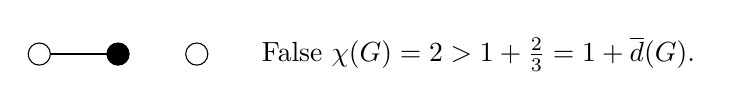
\begin{tikzpicture}
        \draw[] (0,0) -- (1,0);
        
        \draw[fill=white] (0,0) circle (4pt);
        \draw[fill=black] (1,0) circle (4pt);
        \draw[] (2,0) circle (4pt) node[right]{\qquad False $\chi(G) = 2 > 1+\frac{2}{3} = 1+\overline{d}(G).$};
    \end{tikzpicture}
\end{center}




\end{document}